%!TEX root = draft.tex


\section{Empirical Analysis}
\label{sec:Empirical Analysis}
\begin{figure*}[!t]
 \centering
 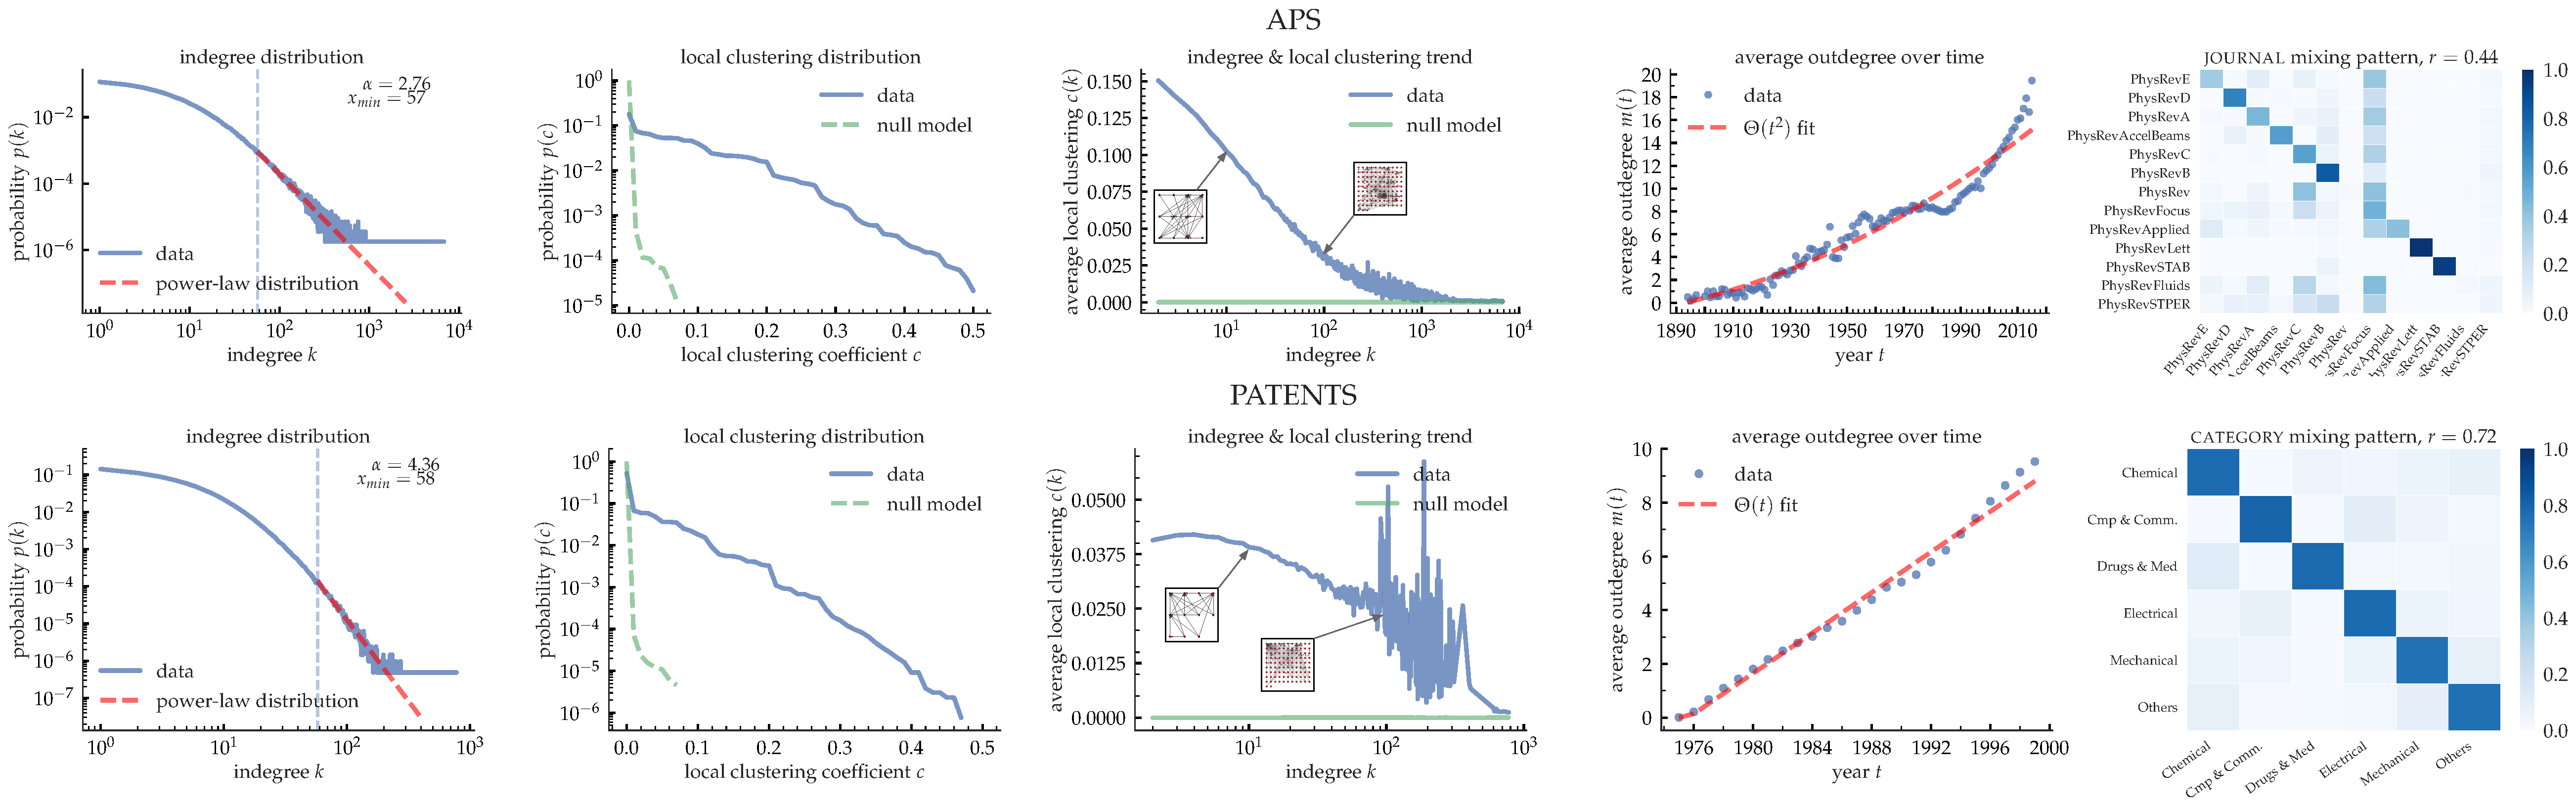
\includegraphics[width=.95\textwidth]{analysis}
 \caption{
 Structural and content properties of \texttt{APS} and \texttt{Patents}.
 The subplots show that citation networks exhibit similar characteristics:
 heavy-tailed indegree distribution, skewed
 local clustering distribution, decreasing indegree \&
 clustering relationship, increasing average outdegree over time and assortative mixing.
 Furthermore, the subplots illustrate that indegree distributions are lognormally distributed
 and networks generated by the null (configuration) model do not exhibit the local clustering
 observed in citation networks.
 % power law fits do not explain indegree distributions in entirety and
 % the null (configuration) model does not exhibit the clustering observed in citation networks.
}
 \label{fig:empirical_analysis}
 \vspace{-4mm}
\end{figure*}

In this section, we show that global structural properties of citation networks
exhibit similar characteristics. Specifically, we identify
regularities in indegree distribution, network growth rate, clustering and
mixing patterns of the seven citation networks described in~\Cref{sub:Datasets}.
Figure \ref{fig:empirical_analysis} illustrates the aforementioned properties of two
attributed networks --- \texttt{APS} and \texttt{Patents}.
% We conclude
% this section by motivating the need to develop edge formation mechanisms
% that can jointly explain the formation of these global network properties over
% time.


% Figure: indegree distributions w. power law fits
Citation networks exhibit highly skewed, heavy tailed indegree distributions.
In~\Cref{fig:empirical_analysis}, we observe that unlike the power law
distribution, lognormal fits accurately describe the degree distribution of two
citation networks --- \texttt{APS} and \texttt{Patents} --- in entirety.
Moreover, a recent study \cite{broido2018scale} on nearly thousand network
datasets provides empirical evidence for the prevalence of lognormal degree
distributions: In 88\% of the cases, the lognormal fits degree distributions as
well as the power law distribution. In~\Cref{sec:Experiments}, we show that
preferential attachment models
\cite{dorogovtsev2000structure,barabasi1999emergence}, which define edge
formation as a function of node degree, can produce networks with realistic
degree distributions, but cannot preserve other properties such as clustering
and homophily.

% Citation networks exhibit highly skewed, heavy tailed indegree distributions.
% % This suggests that most papers receive zero or a few citations, but a small
% % but significant fraction of the nodes turn into popular hubs that receive many citations.
% In~\Cref{fig:empirical_analysis}, we observe that unlike the power
% law distribution, lognormal fits accurately describe the degree distribution of
% two citation networks --- \textsc{aps} and \textsc{patents} --- in entirety.
% Empirical measurements \cite{jeong2003measuring} on real-world networks
% substantiate the preferential attachment phenomenon by showing that popular,
% higher degree nodes are more likely to receive new links. Moreover, the extent
% to which node popularity influences underlying edge formation mechanisms
% directly effects the degree distribution of a network.
% In~\Cref{sec:Experiments}, we show that models
% \cite{dorogovtsev2000structure,barabasi1999emergence} which define edge
% formation as a function of node degree to account for node popularity can
% produce networks with realistic degree distributions, but cannot preserve other
% properties such as clustering and homophily.

% Figure: networks increasing outdegree vs. time + polynomial function fit
The average outdegree of nodes that join real-world networks tends to increase
as functions of network size and time. This phenomenon densifies networks and shrinks their
diameter over time; Leskovec et al. \cite{leskovec2005graphs} show that
densification in many real networks exhibit a power law relationship between the
number of edges $e(t)$ and nodes $n(t)$ at time $t$: $e(t) \propto
n(t)^{\alpha}$. ~\Cref{table:netstats} lists the power law exponent $\alpha$ in
the network datasets. In our proposed model, the outdegree of nodes, which
sequentially join the network, increases at a linear or superlinear rate to accurately
model the accelerated network growth observed in real networks, as shown in ~\Cref{fig:empirical_analysis}.

\begin{table}[H]
 \center
 \caption{Network properties: Densification Power Law (\texttt{DPL}) exponent $\alpha$,
 average local clustering coefficient (\texttt{CC}) and assortativity coefficient
 $r$ of seven citation networks.}
 \label{table:netstats}
 {
  \begin{tabular}[c]{lrrr} \toprule
  Network &  \texttt{DPL} exponent $\alpha$       & Avg. local \texttt{CC}  & Assortativity $r$  \\ \midrule
  \texttt{USSC}         & 2.323     & 0.1159    & -    \\
  \texttt{HEP-PH}       & 1.665     & 0.1203    & -   \\
  \texttt{Semantic}     & 1.584     & 0.0618    & -   \\   \midrule
  \texttt{ACL}          & 1.432     & 0.0655    & 0.067   \\
  \texttt{PYPI}         & 1.208     & 0.0524    & 0.692   \\
  \texttt{APS}          & 1.259     & 0.1084    & 0.443   \\
  \texttt{Patents}      & 1.944     & 0.0414    & 0.721   \\
   \bottomrule
  \end{tabular}
 }
\end{table}

% Clustering coefficient (in table)
High average local clustering is a common characteristic of real-world networks
across disciplines, as shown in~\Cref{table:netstats}. Local clustering
quantifies the extent to which triadic closure influences underlying edge
formation mechanisms. Coupled with small average path length, it also leads to
the small-world phenomenon, in which two randomly picked nodes in large, sparse
real networks are connected by a short path with high probability. Additionally, as shown in~\Cref{fig:empirical_analysis},
the distribution over local clustering in citation networks is highly skewed. Interestingly, our experiments
in~\Cref{sec:Experiments} show that models \cite{klemm2002highly,holme2002growing} that generate
networks with tunable \textit{average} local clustering do not preserve the skewed clustering
distributions of real networks. Furthermore, we observe that the average local clustering decreases as indegree increases.
That is, low indegree nodes tend to have
small, tightly knit neighborhoods and high indegree nodes tend to have large,
star-shaped neighborhoods, as shown
in~\Cref{fig:empirical_analysis}.
% In~\Cref{sec:Proposed Model}, we propose a resource constrained model and explain why resource constraints
% can help in accurately preserving the skewness in the clustering distribution and the degree-clustering relationship.

All four attributed network datasets --- \texttt{ACL}, \texttt{PYPI}, \texttt{APS}
\& \texttt{Patents} --- exhibit homophily; The assortativity coefficients of
these networks range from $0.07$ to $0.72$. As shown in~\Cref{fig:empirical_analysis},
a majority of the edges are between nodes with the same attribute value. Our model,
described in~\Cref{sec:Proposed Model}, can generate heterophilic or homophilic
networks with varying assortativity.

% Conclusion
To summarize, citation networks are homophilic, small-world networks that
undergo accelerated network growth. These networks exhibit heavy tailed indegree
distributions, skewed local clustering distributions, negatively correlated
degree-clustering relationship and assortativity $r > 0$. The regularities in
the  global structure of citation networks perhaps suggest that individuals use
a similar edge formation mechanism. In the next section, we propose a growth
model that can jointly explain the emergence of these structural properties
using a single, resource-constrained edge formation mechanism.

% prompt the question of whether local edge formation mechanisms used by individuals
% is similar as well.

%  similarity of citation
% networks prompts the question - do individuals use the same criteria to form
% edges?


% The skewness and high variance of local clustering in real networks suggests
% that the average local clustering coefficient is not a representative
% statistic, despite its widespread usage.
% By
% explicitly accounting for the fact that nodes are likely to link to neighbors of
% nodes it has already linked to, our model can not only generate networks with
% high average clustering but also capture the local clustering distribution
% observed in real networks.
% In~\Cref{sec:Proposed Model} and~\Cref{sec:Experiments}, we show that our proposed
% edge formation mechanism can intuitively explain the emergence of the skewed
% clustering distribution observed in real networks.
% Indegree-clustering (new property; linear function fit cc = a-bk
%
% In~\Cref{fig:empirical_analysis}, we show
% that the degree-clustering relation in APS and USSC initially decreases as a
% linear function of the logarithmic value of indegree.

%
%  In~\Cref{sec:Experiments}, we show that
% well-known growth models that generate networks with tunable average clustering
% are not flexible enough to explain the degree-clustering trend shown
% in~\Cref{fig:empirical_analysis}.

% Average path length
% Citation networks are clustered, sparse networks that exhibit small average path
% length.~\Cref{table:netstats} lists the average path length (APL) of
% all citation networks. We use a Monte Carlo method \cite{leskovec2008planetary} to estimate the average
% path lengths as the citation networks are prohibitively large.

% In~\Cref{sec:Proposed Model}, we propose
% a growth model in which nodes employ random walks, which are inherently biased towards high degree nodes, to \textit{locally}
% explore the network and probabilistically link to visited nodes.

%
%
%  Generative processes
% based on preferential attachment typically model edge formation
% as a function of node degree. While these models can generate networks with
% power law \cite{barabasi1999emergence} and/or lognormal \cite{van2011lognormal} degree distributions, they disregard
%
% While generative processes based on preferential attachment can produce networks with
% power law \cite{barabasi1999emergence} and/or lognormal \cite{van2011lognormal} degree distributions,

% structural property is important because it helps test the extent to which
% popularity influences underlying edge formation mechanisms.~\Cref{fig:empirical_analysis} shows the observed indegree distribution along with its power law fit for each citation
% network in blue and red respectively. While the power law fits can explain the
% heavy tail, it does not capture the initial concavity in the observed distribution. In~\Cref{sec:Experiments}, we show that our growth model can accurately capture
% the indegree distributions of citation networks in entirety.
